\chapter{Class Diagram}

\begin{figure}[!h]
    \centering
    \includegraphics[page=2,scale=3.2]{pdfs/Boundary.pdf}
    \caption{Boundary}\label{Boundary1}
\end{figure}

\begin{figure}[!h]
    \centering
    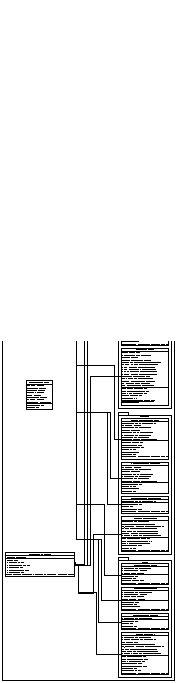
\includegraphics[page=1,scale=4.5]{pdfs/Boundary.pdf}
    \caption{Boundary}\label{Boundary2}
\end{figure}

\begin{figure}[!h]
    \centering
    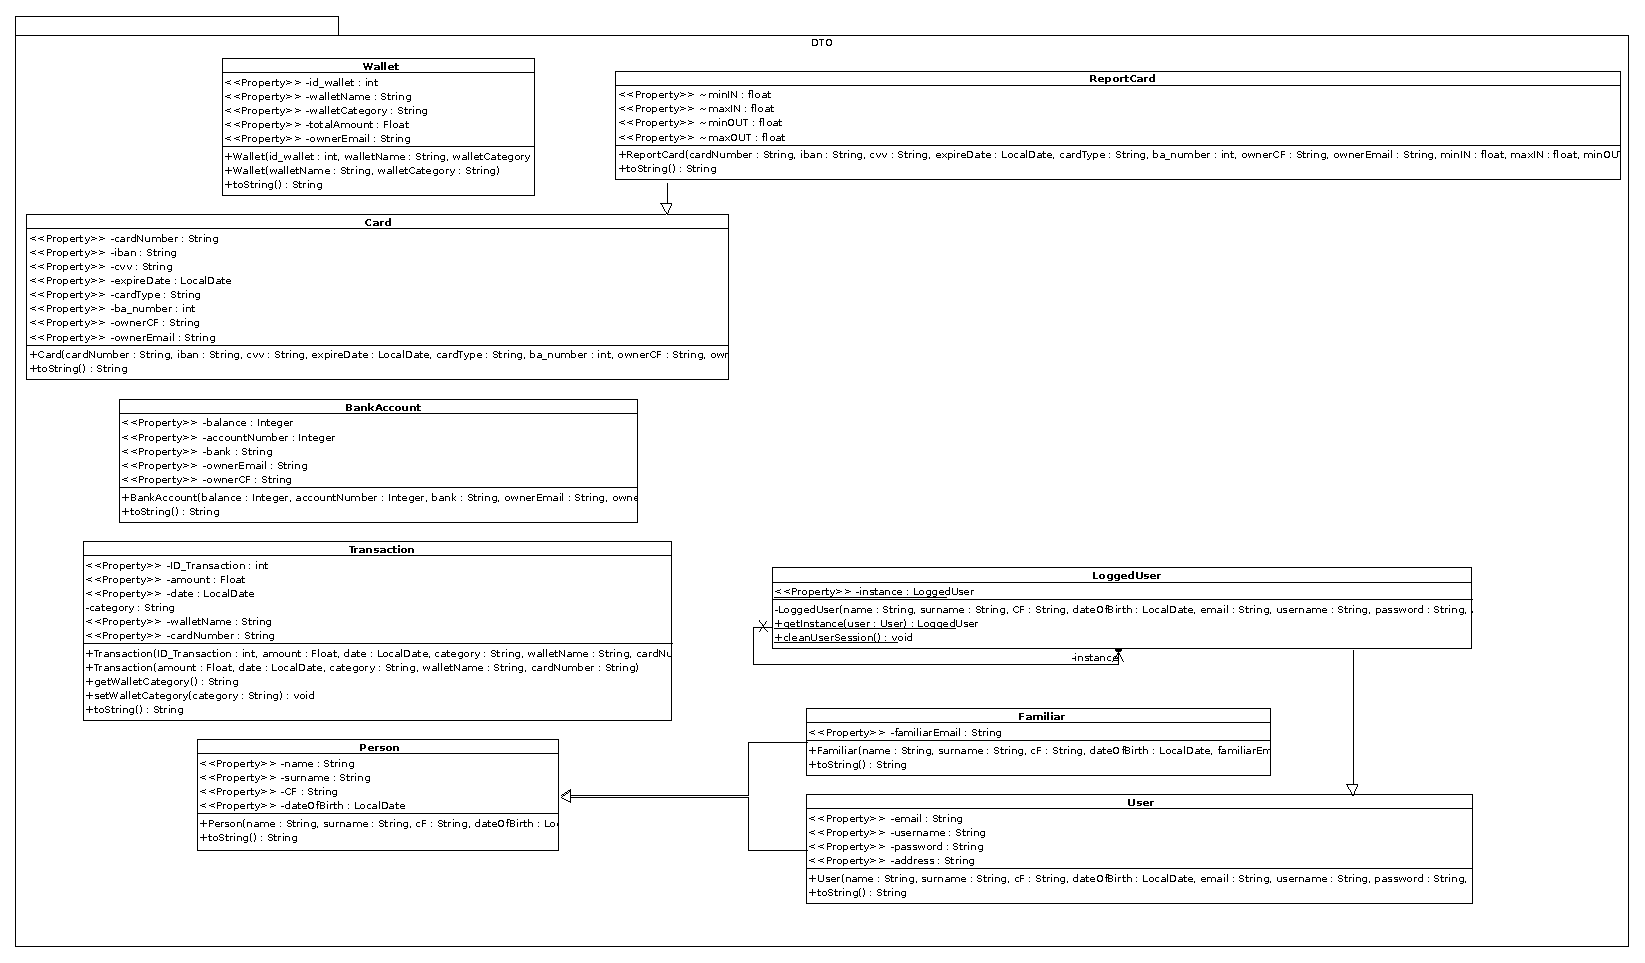
\includegraphics[scale=0.6]{pdfs/DTO.pdf}
    \caption{DTO}\label{DTO}
\end{figure}

\begin{figure}[!h]
    \centering
    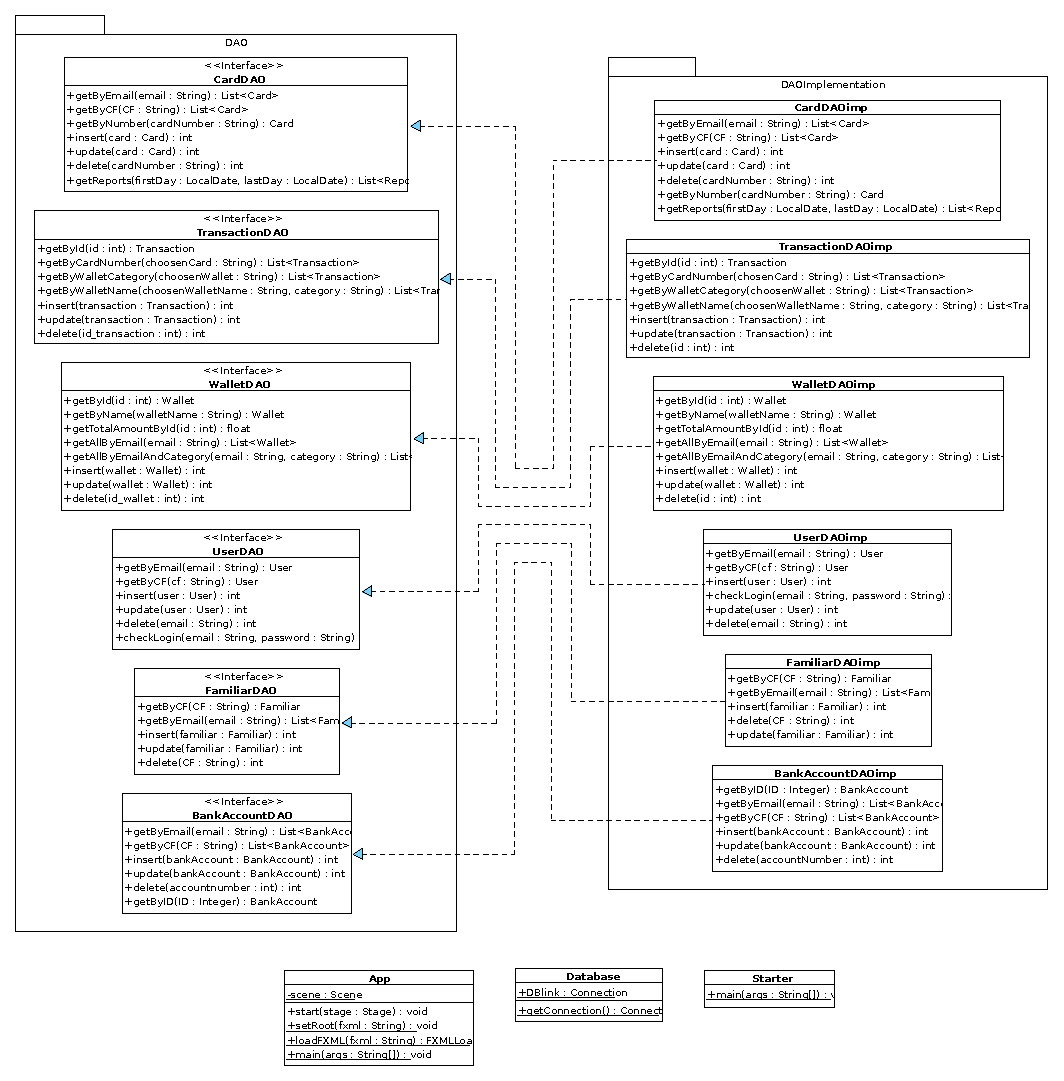
\includegraphics[scale=0.9]{pdfs/DAO.pdf}
    \caption{DAO}\label{DAO}
\end{figure}

\begin{figure}[!h]
    \centering
    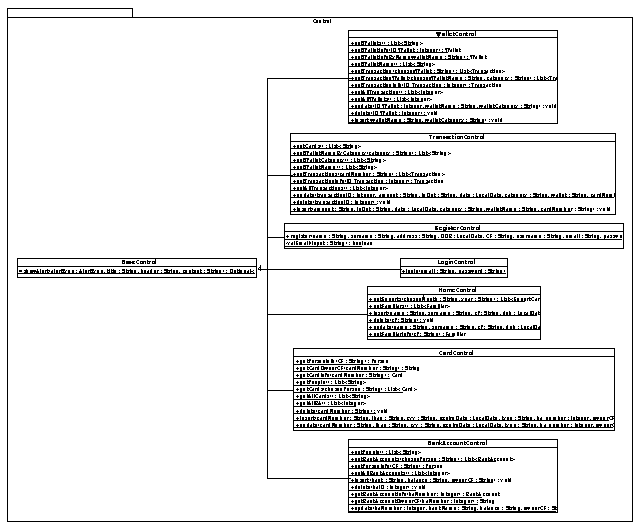
\includegraphics[scale=1.5]{pdfs/Control.pdf}
    \caption{Control}\label{Control}
\end{figure}